\chapter{Estado del arte \label{cap:EstadoDelArte}}

En este capítulo se presenta una revisión de la literatura académica relevante para la detección de noticias falsas y fraude digital, con un enfoque en las técnicas computacionales y los recursos disponibles para el idioma español.

\section{Metodología de Búsqueda}
\label{sec:busqueda_literatura}

La selección de los artículos, investigaciones, trabajos y tesis se efectuó con el apoyo de diversas fuentes y bases de datos académicas, entre las que se incluyen Google Scholar, Semantic Scholar, Nature, IOPscience, MDPI y Web of Science (WoS). La búsqueda se realizó utilizando una combinación de las siguientes palabras clave:

\begin{itemize}
    \item \textit{Spanish fake news}
    \item \textit{Fake news detection techniques}
    \item \textit{Fake news detection language models}
    \item \textit{Employment fraud}
    \item \textit{Labour fraud}
    \item \textit{Heuristic fake news}
    \item \textit{Simulated annealing fake news}
\end{itemize}

A partir de esta búsqueda sistemática, se identificaron y filtraron los trabajos más pertinentes para los objetivos de esta tesis, los cuales se resumen en las Tablas organizadas temáticamente de la \ref{tab:articulos_metodologia} a la \ref{tab:articulos_diversos}.

\section{Clasificación Temática de la Literatura}
\label{sec:clasificacion_tematica}

La literatura revisada se organizó en categorías temáticas para facilitar el análisis y comprensión de las diferentes líneas de investigación. A continuación se presentan los 68 trabajos más relevantes clasificados según su enfoque principal.

\subsection{Artículos sobre Metodología y Corpus de Datos}

Esta categoría agrupa los trabajos fundamentales que se centran en la creación de datasets, metodologías de evaluación y marcos experimentales para la detección de noticias falsas en español.

\begin{table}[htbp]
\centering
\adjustbox{width=\textwidth,center}{%
\small
\begin{tabular}{|l|l|l|c|c|}
\hline
\rowcolor{UAMPurple!20}
\textbf{Título del Artículo} & \textbf{Autores} & \textbf{Publicación} & \textbf{Año} & \textbf{Ref.} \\
\hline
\begin{tabular}[t]{@{}l@{}}Construcción de un dataset de noticias para el\\entrenamiento y evaluación de clasificadores\end{tabular} & Acosta, F. A. Z. & U. Politécnica de Madrid & 2019 & \cite{acosta2019construccion} \\
\hline
\begin{tabular}[t]{@{}l@{}}Overview of the CLEF-2023 CheckThat!\\Lab Task 1\end{tabular} & Alam, F., et al. & CEUR Workshop Proc. & 2023 & \cite{alam2023overview} \\
\hline
\begin{tabular}[t]{@{}l@{}}Overview of mex-a3t at iberlef 2020:\\Fake news and aggressiveness analysis\end{tabular} & Aragón, M. E., et al. & IberLEF Workshop & 2020 & \cite{aragon2020overview} \\
\hline
The CLEF-2023 CheckThat! Lab & Barrón-Cedeño, A., et al. & ECIR 2023 & 2023 & \cite{barron2023clef} \\
\hline
\begin{tabular}[t]{@{}l@{}}Overview of FakeDeS at IberLEF 2021:\\Fake News Detection in Spanish\end{tabular} & Gómez-Adorno, H., et al. & Procesamiento del Lenguaje Natural & 2021 & \cite{gomez2021overview} \\
\hline
\begin{tabular}[t]{@{}l@{}}Detection of fake news in a new corpus for\\the Spanish language\end{tabular} & Posadas-Durán, J. P., et al. & J. of Intelligent and Fuzzy Systems & 2019 & \cite{posadas2019detection} \\
\hline
\begin{tabular}[t]{@{}l@{}}The Spanish Fake News Corpus\\Version 2.0 en GitHub\end{tabular} & Ramírez Cruz, J. M., et al. & GitHub & 2021 & \cite{ramirez2021spanish} \\
\hline
\begin{tabular}[t]{@{}l@{}}Detection of False Information in Spanish\\Using Machine Learning Techniques\end{tabular} & Tretiakov, A., et al. & Springer & 2022 & \cite{tretiakov2022detection} \\
\hline
\end{tabular}
}
\caption{Artículos sobre metodología y corpus de datos.}
\label{tab:articulos_metodologia}
\end{table}

\clearpage

\subsection{Artículos sobre Modelos de Lenguaje y Transformers}

Esta sección incluye los trabajos fundamentales sobre modelos de lenguaje pre-entrenados, arquitecturas transformer y sus aplicaciones en la detección de desinformación.

\begin{table}[htbp]
\centering
\adjustbox{width=\textwidth,center}{%
\small
\begin{tabular}{|l|l|l|c|c|}
\hline
\rowcolor{UAMPurple!20}
\textbf{Título del Artículo} & \textbf{Autores} & \textbf{Publicación} & \textbf{Año} & \textbf{Ref.} \\
\hline
\begin{tabular}[t]{@{}l@{}}Constitutional AI: Harmlessness\\from AI Feedback\end{tabular} & Bai, Y., et al. & arXiv & 2022 & \cite{bai2022constitutional} \\
\hline
\begin{tabular}[t]{@{}l@{}}Enhancing Misinformation Detection in Spanish\\with BERT and RoBERTa\end{tabular} & Blanco-Fernández, Y., et al. & Applied Sciences & 2024 & \cite{blanco2024enhancing} \\
\hline
\begin{tabular}[t]{@{}l@{}}Language Models are Few-Shot Learners\\(GPT-3)\end{tabular} & Brown, T. B., et al. & arXiv & 2020 & \cite{brown2020language} \\
\hline
\begin{tabular}[t]{@{}l@{}}BERT: Pre-training of Deep Bidirectional\\Transformers for Language Understanding\end{tabular} & Devlin, J., et al. & arXiv & 2018 & \cite{devlin2018bert} \\
\hline
\begin{tabular}[t]{@{}l@{}}Gemini: A Family of Highly Capable\\Multimodal Models\end{tabular} & Gemini Team, Google & arXiv & 2023 & \cite{gemini2023family} \\
\hline
\begin{tabular}[t]{@{}l@{}}Bad Actor, Good Advisor: Exploring the Role of\\LLMs in Fake News Detection\end{tabular} & Hu, B., et al. & AAAI Conference & 2024 & \cite{hu2024bad} \\
\hline
\begin{tabular}[t]{@{}l@{}}TinyBERT: Distilling BERT for Natural\\Language Understanding\end{tabular} & Jiao, X., et al. & arXiv & 2019 & \cite{jiao2019tinybert} \\
\hline
\begin{tabular}[t]{@{}l@{}}Fake News Detection in Spanish Using\\Deep Learning Techniques\end{tabular} & Martínez-Gallego, K., et al. & arXiv & 2021 & \cite{martinez2021fake} \\
\hline
\begin{tabular}[t]{@{}l@{}}DistilBERT, a distilled version of BERT:\\smaller, faster, cheaper and lighter\end{tabular} & Sanh, V., et al. & arXiv & 2019 & \cite{sanh2019distilbert} \\
\hline
\begin{tabular}[t]{@{}l@{}}Improving multiclass classification of fake\\news using BERT-Based models\end{tabular} & Shushkevich, E., et al. & Inventions & 2023 & \cite{shushkevich2023improving} \\
\hline
\begin{tabular}[t]{@{}l@{}}Adapting fake news detection to the era\\of large language models\end{tabular} & Su, J., et al. & arXiv & 2023 & \cite{su2023adapting} \\
\hline
\begin{tabular}[t]{@{}l@{}}Fake news detectors are biased against texts\\generated by large language models\end{tabular} & Su, J., et al. & arXiv & 2023 & \cite{su2023fake} \\
\hline
\begin{tabular}[t]{@{}l@{}}LLaMA: Open and Efficient Foundation\\Language Models\end{tabular} & Touvron, H., et al. & arXiv & 2023 & \cite{touvron2023llama} \\
\hline
\begin{tabular}[t]{@{}l@{}}Attention is All You Need\\(Transformers)\end{tabular} & Vaswani, A., et al. & arXiv & 2017 & \cite{vaswani2017attention} \\
\hline
\begin{tabular}[t]{@{}l@{}}Evaluation of Fake News Detection with\\Knowledge-Enhanced Language Models\end{tabular} & Whitehouse, C., et al. & arXiv & 2022 & \cite{whitehouse2022evaluation} \\
\hline
\end{tabular}
}
\caption{Artículos sobre modelos de lenguaje y transformers.}
\label{tab:articulos_modelos_lenguaje}
\end{table}

\clearpage

\subsection{Artículos sobre Técnicas Metaheurísticas y Optimización}

Esta categoría incluye trabajos que emplean algoritmos metaheurísticos, optimización de hiperparámetros y enfoques de optimización para la detección de noticias falsas y fraude.

\begin{table}[htbp]
\centering
\adjustbox{width=\textwidth,center}{%
\small
\begin{tabular}{|l|l|l|c|c|}
\hline
\rowcolor{UAMPurple!20}
\textbf{Título del Artículo} & \textbf{Autores} & \textbf{Publicación} & \textbf{Año} & \textbf{Ref.} \\
\hline
\begin{tabular}[t]{@{}l@{}}Diseño y desarrollo de un método\\heurístico basado en un sistema socio-cultural\end{tabular} & Anselmo, M. G. R. & UNAM & 2013 & \cite{anselmo2013diseno} \\
\hline
\begin{tabular}[t]{@{}l@{}}Modeling and solving the fake news\\detection scheduling problem\end{tabular} & Aqil, S., \& Lahby, M. & Studies in Comp. Intelligence & 2021 & \cite{aqil2021modeling} \\
\hline
\begin{tabular}[t]{@{}l@{}}On the Benefits of Using Metaheuristics\\in Hyperparameter Tuning\end{tabular} & Bacanin, N., et al. & Energies & 2023 & \cite{bacanin2023benefits} \\
\hline
\begin{tabular}[t]{@{}l@{}}A heuristic-driven uncertainty-based\\ensemble framework for fake news detection\end{tabular} & Das, S. D., et al. & Neurocomputing & 2022 & \cite{das2022heuristic} \\
\hline
\begin{tabular}[t]{@{}l@{}}Unmasking deception: a CNN and adaptive\\PSO approach to detecting fake online reviews\end{tabular} & Deshai, N., \& Rao, B. B. & Soft Computing & 2023 & \cite{deshai2023unmasking} \\
\hline
\begin{tabular}[t]{@{}l@{}}Financial Statement Fraud Detection in\\Indonesia using Meta-Heuristics\end{tabular} & Hidayattullah, S., et al. & IWBIS & 2020 & \cite{hidayattullah2020financial} \\
\hline
\begin{tabular}[t]{@{}l@{}}Gaussian Process Regression's Hyperparameters\\Optimization to Predict Financial Distress\end{tabular} & Horak, J., \& Sabek, A. & Retos & 2023 & \cite{horak2023gaussian} \\
\hline
\begin{tabular}[t]{@{}l@{}}Calibración de hiper-parámetros en algoritmos\\metaheurísticos para la detección de fraude digital\end{tabular} & Hurtado Avilés, G., et al. & BUAP & 2024 & \cite{hurtado2024calibracion} \\
\hline
\begin{tabular}[t]{@{}l@{}}Variable neighborhood search for weighted total\\domination problem\end{tabular} & Kapunac, S., et al. & Applied Soft Computing & 2023 & \cite{kapunac2023variable} \\
\hline
\begin{tabular}[t]{@{}l@{}}Ensemble effort estimation with metaheuristic\\hyperparameters and weight optimization\end{tabular} & Yasmin, A., et al. & PLOS ONE & 2024 & \cite{yasmin2024ensemble} \\
\hline
\begin{tabular}[t]{@{}l@{}}Improving fake news detection using K-Means\\and support vector machine approaches\end{tabular} & Yazdi, K. M., et al. & Waset & 2020 & \cite{yazdi2020improving} \\
\hline
\begin{tabular}[t]{@{}l@{}}A novel hybrid multi-thread metaheuristic\\approach for fake news detection\end{tabular} & Yildirim, G. & Applied Intelligence & 2023 & \cite{yildirim2023novel} \\
\hline
\begin{tabular}[t]{@{}l@{}}Using large language models for\\hyperparameter optimization\end{tabular} & Zhang, M. R., et al. & openreview.net & 2023 & \cite{zhang2023using} \\
\hline
\end{tabular}
}
\caption{Artículos sobre técnicas metaheurísticas y optimización.}
\label{tab:articulos_metaheuristicas}
\end{table}

\clearpage

\subsection{Artículos sobre Revisiones y Estudios Comprehensivos}

Esta sección agrupa las revisiones sistemáticas, surveys y estudios comprehensivos que analizan el estado del arte en detección de noticias falsas y técnicas relacionadas.

\begin{table}[htbp]
\centering
\adjustbox{width=\textwidth,center}{%
\small
\begin{tabular}{|l|l|l|c|c|}
\hline
\rowcolor{UAMPurple!20}
\textbf{Título del Artículo} & \textbf{Autores} & \textbf{Publicación} & \textbf{Año} & \textbf{Ref.} \\
\hline
A survey on fake news and rumour\\detection techniques & Bondielli, A., \& Marcelloni, F. & Information Sciences & 2019 & \cite{bondielli2019survey} \\
\hline
Deep learning for fake news detection:\\A comprehensive survey & Hu, L., et al. & AI Open & 2022 & \cite{hu2022deep} \\
\hline
\begin{tabular}[t]{@{}l@{}}A Comprehensive Review on Fake News\\Detection With Deep Learning\end{tabular} & Mridha, M. F., et al. & IEEE Access & 2021 & \cite{mridha2021comprehensive} \\
\hline
\begin{tabular}[t]{@{}l@{}}A comprehensive review on automatic\\detection of fake news on social media\end{tabular} & Singh, M. K., et al. & Multimedia Tools and Applications & 2023 & \cite{singh2023comprehensive} \\
\hline
Fake News Detection: A Deep Learning\\Approach & Thota, A., et al. & SMU Scholar & 2018 & \cite{thota2018fake} \\
\hline
\end{tabular}
}
\caption{Artículos sobre revisiones y estudios comprehensivos.}
\label{tab:articulos_revisiones}
\end{table}

\subsection{Artículos sobre Detección de Fraude Financiero y Laboral}

Esta categoría incluye trabajos específicos sobre la detección de fraude en contextos financieros, laborales y comerciales.

\begin{table}[htbp]
\centering
\adjustbox{width=\textwidth,center}{%
\small
\begin{tabular}{|l|l|l|c|c|}
\hline
\rowcolor{UAMPurple!20}
\textbf{Título del Artículo} & \textbf{Autores} & \textbf{Publicación} & \textbf{Año} & \textbf{Ref.} \\
\hline
El fraude en México: daños patrimoniales y\\trabajo legislativo para enfrentarlo & Aguirre Quezada, J. P. & Senado de México & 2023 & \cite{aguirre2023fraude} \\
\hline
Fraude laboral en la era digital & Alvarez, O. H. & Rev. Gen. de Derecho del Trabajo & 2021 & \cite{alvarez2021fraude} \\
\hline
Corporate employment, red flags, and\\audit effort & Cao, J., et al. & J. of Accounting and Public Policy & 2020 & \cite{cao2020corporate} \\
\hline
Online Recruitment Fraud Detection using ANN & Nasser, I. M., et al. & PICICT & 2021 & \cite{nasser2021online} \\
\hline
\begin{tabular}[t]{@{}l@{}}Proyecto de seguridad para reducir fraudes y\\robos en Marketplace de Facebook\end{tabular} & Osorio-Giraldo, J. M., et al. & Coloquio de Inv. Formativa & 2023 & \cite{osorio2023proyecto} \\
\hline
\begin{tabular}[t]{@{}l@{}}Selección de una técnica de aprendizaje de\\máquina para la detección de Fraude Financiero\end{tabular} & Villamil Arcos, C. & U. Nacional de Colombia & 2022 & \cite{villamil2022seleccion} \\
\hline
\end{tabular}
}
\caption{Artículos sobre detección de fraude financiero y laboral.}
\label{tab:articulos_fraude}
\end{table}

\clearpage

\subsection{Artículos sobre Análisis de Comportamiento Social y Heurísticas}

Esta sección incluye trabajos que analizan el comportamiento humano, heurísticas cognitivas y factores sociales en la propagación y percepción de noticias falsas.

\begin{table}[htbp]
\centering
\adjustbox{width=\textwidth,center}{%
\small
\begin{tabular}{|l|l|l|c|c|}
\hline
\rowcolor{UAMPurple!20}
\textbf{Título del Artículo} & \textbf{Autores} & \textbf{Publicación} & \textbf{Año} & \textbf{Ref.} \\
\hline
\begin{tabular}[t]{@{}l@{}}Post-truth propaganda: heuristic processing\\of political fake news on Facebook\end{tabular} & Ali, K., \& Zain-Ul-Abdin, K. & J. Applied Comm. Res. & 2020 & \cite{ali2020posttruth} \\
\hline
\begin{tabular}[t]{@{}l@{}}Fake news on Facebook: examining the\\impact of heuristic cues\end{tabular} & Ali, K., et al. & Internet Research & 2021 & \cite{ali2021fake} \\
\hline
\begin{tabular}[t]{@{}l@{}}Fake news en Chile y España: ¿Cómo los\\medios nos hablan de noticias falsas?\end{tabular} & Cárcamo-Ulloa, L., et al. & J. of Iberian and Latin Am. Res. & 2021 & \cite{carcamo2021fake} \\
\hline
\begin{tabular}[t]{@{}l@{}}Fake news y coronavirus: detección de los\\principales actores y tendencias en Twitter\end{tabular} & Pérez-Dasilva, J., et al. & El Profesional De La Información & 2020 & \cite{perez2020fake} \\
\hline
\begin{tabular}[t]{@{}l@{}}A New Application of Social Impact in Social\\Media for Overcoming Fake News in Health\end{tabular} & Pulido, C., et al. & Int. J. of Env. Res. and Public Health & 2020 & \cite{pulido2020new} \\
\hline
\begin{tabular}[t]{@{}l@{}}Stylometric fake news detection based on\\natural language processing\end{tabular} & Tsai, C. M. & Electronics & 2023 & \cite{tsai2023stylometric} \\
\hline
\end{tabular}
}
\caption{Artículos sobre análisis de comportamiento social y heurísticas.}
\label{tab:articulos_comportamiento}
\end{table}

\subsection{Artículos sobre Sistemas de Información y Representación de Conocimiento}

Esta categoría agrupa trabajos relacionados con sistemas de información, representación de conocimiento, ontologías y interfaces de consulta.

\begin{table}[htbp]
\centering
\adjustbox{width=\textwidth,center}{%
\small
\begin{tabular}{|l|l|l|c|c|}
\hline
\rowcolor{UAMPurple!20}
\textbf{Título del Artículo} & \textbf{Autores} & \textbf{Publicación} & \textbf{Año} & \textbf{Ref.} \\
\hline
Towards a definition of knowledge graphs & Ehrlinger, L., \& Wöß, W. & SEMANTiCS & 2016 & \cite{ehrlinger2016towards} \\
\hline
\begin{tabular}[t]{@{}l@{}}Interfaz de consulta en idioma español para\\la búsqueda de información\end{tabular} & García Robledo, G. A., et al. & UAM & 2020 & \cite{garcia2020interfaz} \\
\hline
\begin{tabular}[t]{@{}l@{}}Representación ontológica de la arquitectura\\de control de un robot SCARA\end{tabular} & Hurtado Avilés, G., et al. & BUAP & 2024 & \cite{hurtado2024representacion} \\
\hline
Knowledge representation and reasoning & Levesque, H. J. & Annual review of computer science & 1986 & \cite{levesque1986knowledge} \\
\hline
Natural Language Processing & Liddy, E. D. & Syracuse University & 2001 & \cite{liddy2001natural} \\
\hline
\begin{tabular}[t]{@{}l@{}}Sistema de alerta temprana para monitorear\\la propagación de noticias falsas\end{tabular} & Manzano-Velasco, C. E., et al. & Universidad del Cauca & 2024 & \cite{manzano2024sistema} \\
\hline
\begin{tabular}[t]{@{}l@{}}Detección y representación de eventos en\\un ambiente académico inteligente\end{tabular} & Padilla Cuevas, J., et al. & UAM & 2019 & \cite{padilla2019deteccion} \\
\hline
\begin{tabular}[t]{@{}l@{}}Extracción de Información Semántica para la\\Clasificación de Servicios Web\end{tabular} & Reyes-Ortiz, J. A. & CENIDET & 2008 & \cite{reyes2008extraccion} \\
\hline
\begin{tabular}[t]{@{}l@{}}Clinical Decision Support Systems: A Survey\\of NLP-Based Approaches\end{tabular} & Reyes-Ortiz, J. A., et al. & DEXA & 2015 & \cite{reyes2015clinical} \\
\hline
Knowledge representation & Shapiro, S. C. & Encyclopedia of cognitive science & 2006 & \cite{shapiro2006knowledge} \\
\hline
\end{tabular}
}
\caption{Artículos sobre sistemas de información y representación de conocimiento.}
\label{tab:articulos_sistemas}
\end{table}

\clearpage

\section{Análisis Temático de la Literatura Relevante}
\label{sec:analisis_tematico}

Más allá de la clasificación, es fundamental analizar en profundidad las contribuciones clave de cada grupo temático. A continuación, se detallan los aportes más significativos de cada categoría para la planeación y ejecución de la metodología de esta tesis.

\subsection{El Desafío de los Datos: Creación de Corpus en Español}
Un desafío fundamental para el Procesamiento del Lenguaje Natural (PLN) en español es la escasez de conjuntos de datos etiquetados a gran escala. La creación y curación de corpus es, por tanto, una línea de investigación fundamental. El trabajo de Fin de Máster de Zules Acosta \cite{acosta2019construccion} fue uno de los pioneros en este ámbito, centrándose en la creación de un dataset de 598 noticias en castellano. Su investigación destaca la importancia de la \textit{ingeniería de características} para seleccionar estrategias óptimas de extracción que permitan a los modelos de aprendizaje automático clasificar eficazmente la veracidad del contenido \cite{acosta2019construccion}.

Por otro lado, el trabajo de Posadas-Durán et al. \cite{posadas2019detection} introdujo el \textit{Spanish Fake News Corpus} (con 971 noticias), un recurso clave para analizar y detectar información engañosa mediante métodos basados en el estilo de la escritura. Este corpus ha sido fundamental en competencias internacionales como IberLEF, donde se han evaluado diversas metodologías para el español \cite{gomez2021overview}, incluyendo el análisis de agresividad y noticias falsas en el español de México \cite{aragon2020overview}.

Más recientemente, se han publicado corpus de mayor escala que han sido cruciales para esta tesis. Tretiakov et al. \cite{tretiakov2022detection} aportaron un nuevo conjunto de datos con 1,958 noticias falsas en español, mientras que el trabajo de Blanco-Fernández et al. \cite{blanco2024enhancing} introdujo el \textit{Spanish Political Fake News Dataset}. Este último, con más de 57,000 noticias, representa uno de los mayores recursos disponibles y es la fuente principal de datos para esta tesis. La unificación de estos cuatro corpus constituye el fundamento metodológico de este trabajo.

\subsection{Revolución de los Modelos de Lenguaje y Transformers}
La arquitectura Transformer, introducida por Vaswani et al. \cite{vaswani2017attention}, revolucionó el campo del PLN con su mecanismo de atención. Este trabajo fundamental sentó las bases para modelos como BERT \cite{devlin2018bert}, que introdujo el concepto de pre-entrenamiento bidireccional, y sus variantes optimizadas como DistilBERT \cite{sanh2019distilbert} y TinyBERT \cite{jiao2019tinybert}, que buscan reducir el costo computacional manteniendo el rendimiento.

El paradigma de los Grandes Modelos de Lenguaje (LLMs) se consolidó con GPT-3 \cite{brown2020language}, que demostró capacidades emergentes de few-shot learning. Trabajos más recientes como LLaMA \cite{touvron2023llama} han democratizado el acceso a modelos de gran escala, mientras que Gemini \cite{gemini2023family} ha avanzado hacia capacidades multimodales. La investigación en IA Constitucional \cite{bai2022constitutional} ha abordado la alineación y seguridad de estos sistemas.

Para el español específicamente, Martínez-Gallego et al. \cite{martinez2021fake} exploraron la aplicación de BERT y BETO, mientras que Blanco-Fernández et al. \cite{blanco2024enhancing} compararon BERT y RoBERTa para la detección de desinformación. La investigación sobre el rol dual de los LLMs \cite{hu2024bad, su2023adapting, su2023fake} ha revelado tanto oportunidades como desafíos en su aplicación para la detección de noticias falsas.

\subsection{Optimización y Metaheurísticas en la Detección}
Los algoritmos metaheurísticos han demostrado ser herramientas valiosas para abordar problemas complejos de optimización en la detección de noticias falsas. Aqil y Lahby \cite{aqil2021modeling} modelaron la detección como un problema de scheduling, aplicando algoritmos genéticos y optimización por enjambre de partículas. La calibración de hiperparámetros \cite{bacanin2023benefits, hurtado2024calibracion} ha emergido como una aplicación clave, donde las metaheurísticas superan a los métodos tradicionales de grid search.

El enfoque de ensemble con marcos heurísticos \cite{das2022heuristic} ha mostrado prometedores resultados al combinar múltiples modelos con información estadística adicional. Yildirim \cite{yildirim2023novel} propuso un enfoque híbrido multi-thread que optimiza tanto la selección de características como los parámetros del modelo. La aplicación de PSO para la detección de reseñas falsas \cite{deshai2023unmasking} demuestra la versatilidad de estas técnicas más allá de las noticias.

\subsection{Perspectivas Interdisciplinarias y Análisis Social}
La comprensión del fenómeno de las noticias falsas requiere un enfoque interdisciplinario que combine aspectos técnicos con análisis social y psicológico. Ali et al. \cite{ali2021fake, ali2020posttruth} han investigado cómo las heurísticas cognitivas humanas, como la popularidad social (``me gusta''), influyen en la percepción de credibilidad. Su trabajo sobre el procesamiento heurístico durante eventos políticos específicos (elecciones de 2016 en EE.UU.) proporciona insights valiosos sobre la psicología de la desinformación.

El análisis del rol de los medios de comunicación \cite{carcamo2021fake, perez2020fake} ha revelado patrones culturales en cómo diferentes países abordan la desinformación. Pulido et al. \cite{pulido2020new} propusieron el marco SISM (Social Impact in Social Media) para combatir específicamente la desinformación en salud, un dominio crítico durante pandemias.

\subsection{Detección de Fraude: Más Allá de las Noticias}
La investigación se ha extendido hacia otros dominios de fraude digital. En el ámbito laboral, Nasser et al. \cite{nasser2021online} desarrollaron sistemas basados en redes neuronales para detectar ofertas de trabajo fraudulentas, mientras que Alvarez \cite{alvarez2021fraude} analizó las nuevas modalidades de fraude laboral en la era digital latinoamericana.

En el sector financiero, la investigación de Hidayattullah et al. \cite{hidayattullah2020financial} demostró la efectividad de combinar aprendizaje automático con optimización metaheurística para detectar fraudes en estados financieros. Cao et al. \cite{cao2020corporate} establecieron conexiones entre indicadores de empleo corporativo y riesgo de fraude, proporcionando herramientas valiosas para auditores.

\section{Investigación y Desarrollo de Métodos de Detección}

Un gran esfuerzo de la comunidad científica se ha centrado en el desarrollo de métodos automáticos para la detección de noticias falsas. Propuestas como la de Pulido et al. \cite{pulido2020new}, proponen una metodología basada en el análisis de redes sociales, denominada SISM (\textit{Social Impact in Social Media}), para identificar y evaluar la difusión de información falsa en el ámbito de la salud. Por otro lado, revisiones exhaustivas como la de Hu et al. \cite{hu2022deep} analizan el potencial del aprendizaje profundo para detectar patrones sutiles en el lenguaje y el contenido de grandes volúmenes de datos. El Mapa Conceptual \ref{fig:mapa_conceptual_3} ilustra la relación entre los artículos de revisión y aquellos enfocados en análisis de contenido y detección de fraude financiero.

\begin{figure}[h!]
    \centering
    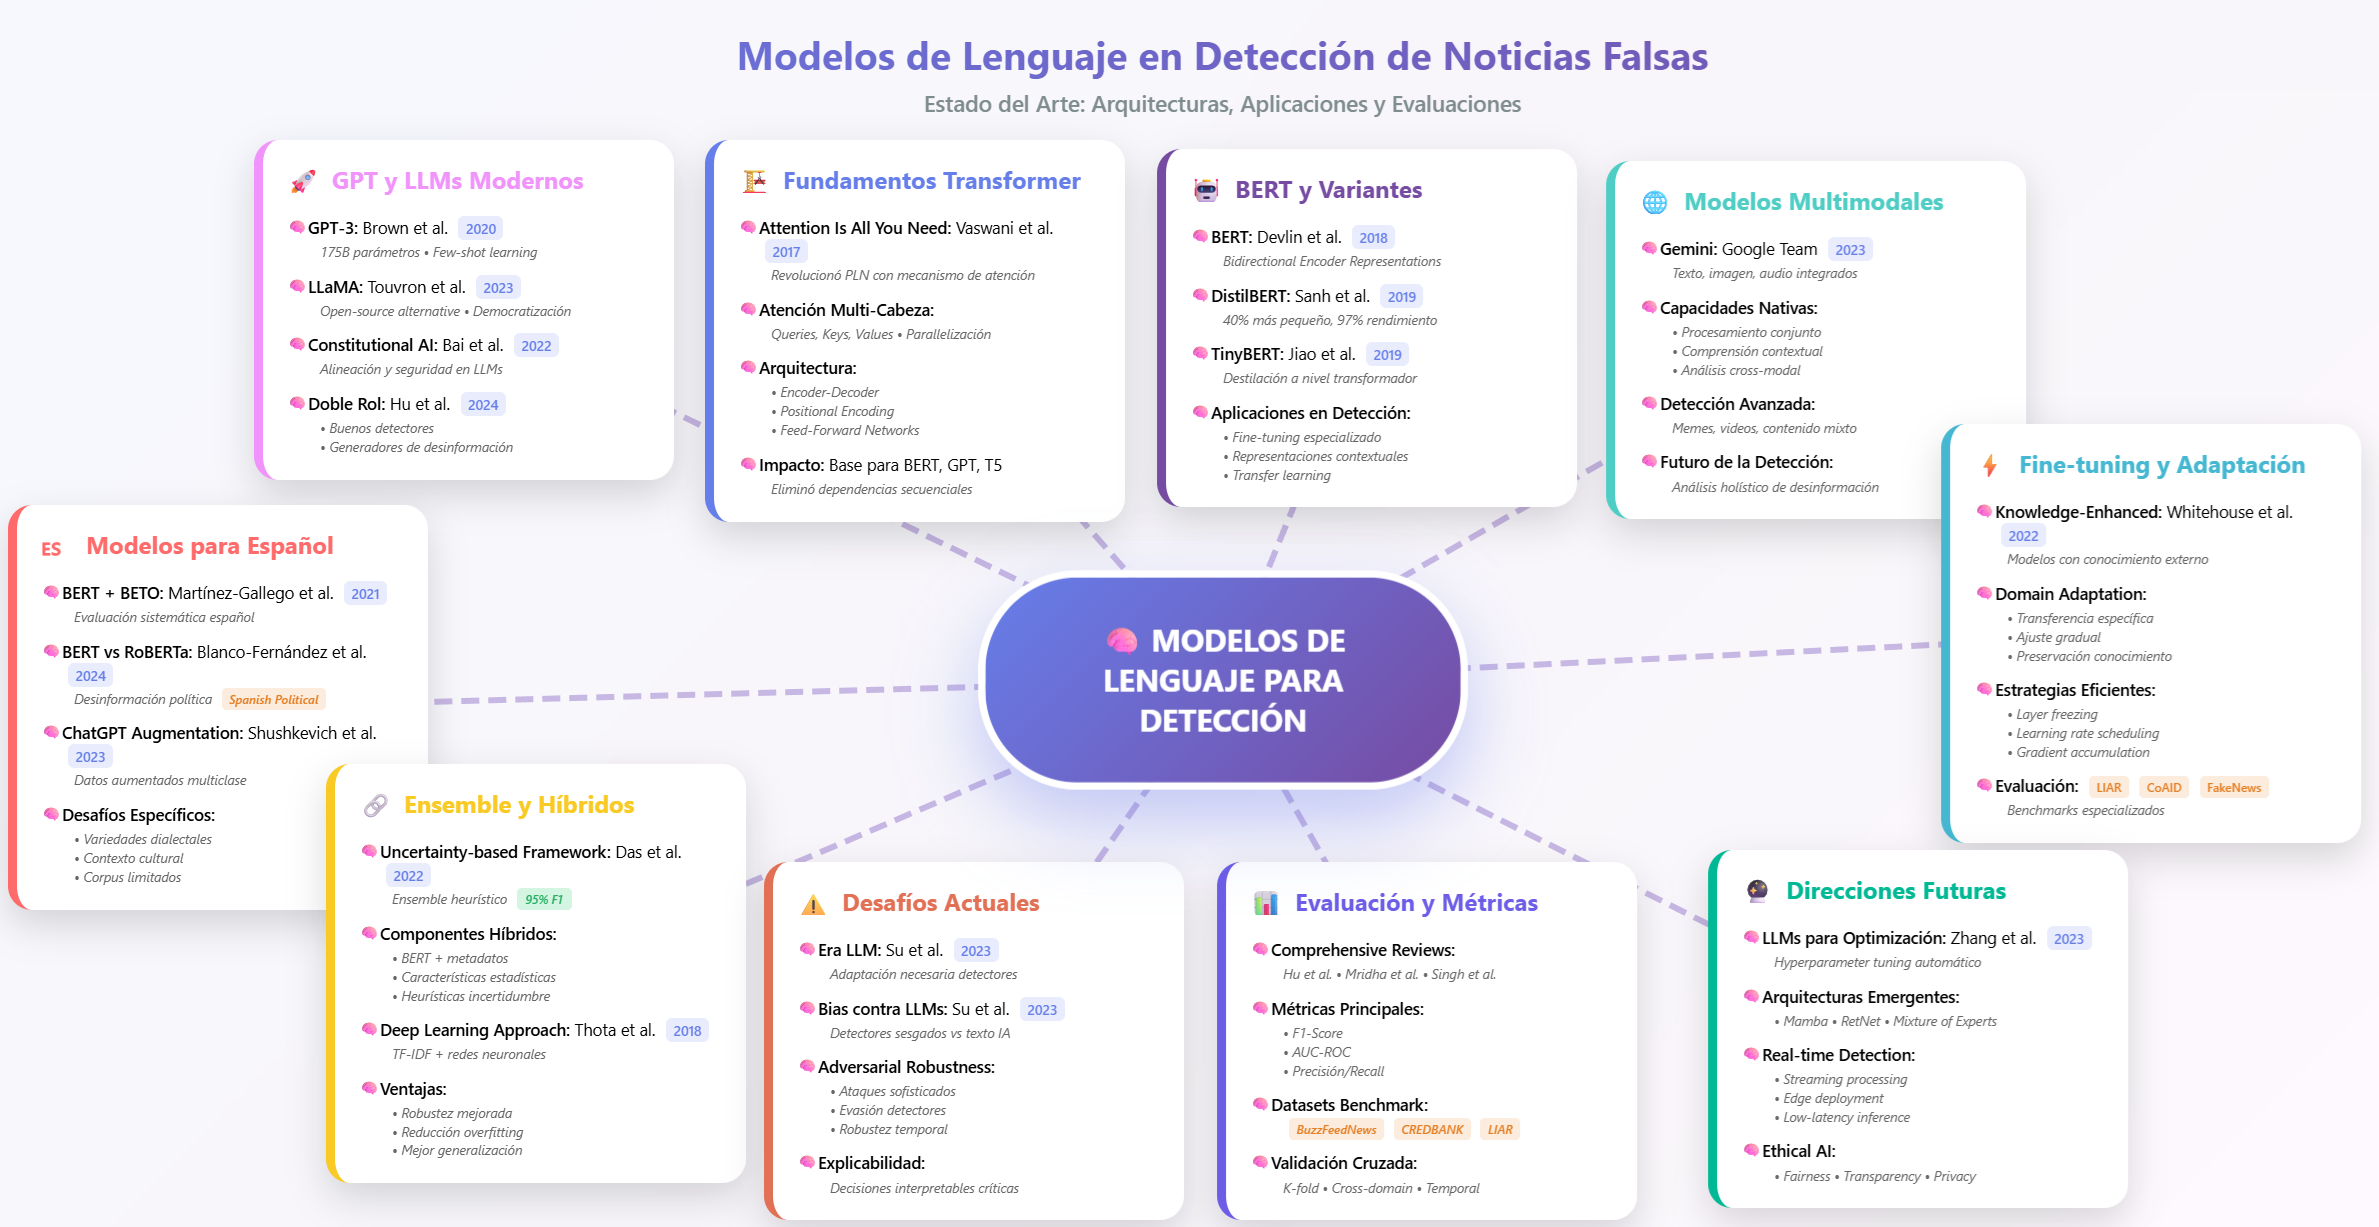
\includegraphics[width=\textwidth]{Imagenes/mapaConceptual3.png}
    \caption{Mapa Conceptual 3: Artículos que son revisiones o están relacionados al análisis de contenido y detección de fraude financiero.}
    \label{fig:mapa_conceptual_3}
\end{figure}

\begin{table}[h!]
\centering
\adjustbox{width=\textwidth,center}{%
\small
\begin{tabular}{|l|l|l|}
\hline
\rowcolor{HeaderBlue!20}
\textbf{Categoría} & \textbf{Contribución Principal} & \textbf{Dataset(s) Mencionados} \\
\hline
NLP & Propone una metodología SISM para combatir noticias falsas en salud \cite{pulido2020new}. & Propio (basado en Twitter). \\
\hline
Revisiones & Revisa exhaustivamente técnicas de Deep Learning (arquitecturas, datasets, métricas) \cite{hu2022deep}. & BuzzFeedNews, LIAR, CREDBANK. \\
\hline
Revisiones & Revisa diferentes enfoques para la detección automática de rumores y noticias falsas \cite{bondielli2019survey}. & Snopes, FactCheck, PolitiFact, etc. \\
\hline
\end{tabular}
}
\caption{Artículos relacionados con la investigación y desarrollo de métodos de detección.}
\label{tab:metodos_deteccion}
\end{table}

\section{Implementación de Soluciones Prácticas}
Diversas iniciativas han buscado poner en práctica los avances teóricos. Posadas-Durán et al. \cite{posadas2019detection} presentaron un nuevo corpus en español y un método de detección basado en el estilo de escritura. Martínez-Gallego et al. \cite{martinez2021fake} exploraron el uso de técnicas de aprendizaje profundo como BERT y BETO para el español. Thota et al. \cite{thota2018fake} presentaron un enfoque similar utilizando un vectorizador TF-IDF en un modelo de Deep Learning. Adicionalmente, Whitehouse et al. \cite{whitehouse2022evaluation} investigaron el impacto de integrar conocimiento externo en los Modelos de Lenguaje Pre-entrenados (PLMs) para mejorar la detección.

\begin{table}[h!]
\centering
\adjustbox{width=\textwidth,center}{%
\small
\begin{tabular}{|l|l|l|}
\hline
\rowcolor{HeaderBlue!20}
\textbf{Categoría} & \textbf{Contribución Principal} & \textbf{Dataset(s) Mencionados} \\
\hline
NLP & \begin{tabular}[t]{@{}l@{}}Propone un método basado en el estilo de escritura para detectar \\ noticias falsas en español \cite{posadas2019detection}.\end{tabular} & \begin{tabular}[t]{@{}l@{}}SpanishFakeNewsCorpus \\ (de GitHub)\end{tabular} \\
\hline
Deep Learning & \begin{tabular}[t]{@{}l@{}}Evalúa diferentes arquitecturas de Deep Learning para la \\ detección de noticias falsas en español, incluyendo BERT y BETO \cite{martinez2021fake}.\end{tabular} & Kaggle Fake/Real News \\
\hline
TF-IDF & \begin{tabular}[t]{@{}l@{}}Utiliza el vectorizador TF-IDF para la representación textual en un \\ modelo de Deep Learning para la detección de noticias falsas \cite{thota2018fake}.\end{tabular} & fakenewschallenge.org \\
\hline
Modelos de Lenguaje & \begin{tabular}[t]{@{}l@{}}Evalúa la detección de noticias falsas con modelos de lenguaje \\ mejorados con conocimiento \cite{whitehouse2022evaluation}.\end{tabular} & LIAR, COVID-19 (newschecker.in) \\
\hline
\end{tabular}
}
\caption{Artículos relacionados a la implementación de soluciones prácticas.}
\label{tab:soluciones_practicas}
\end{table}

\begin{figure}[h!]
    \centering
    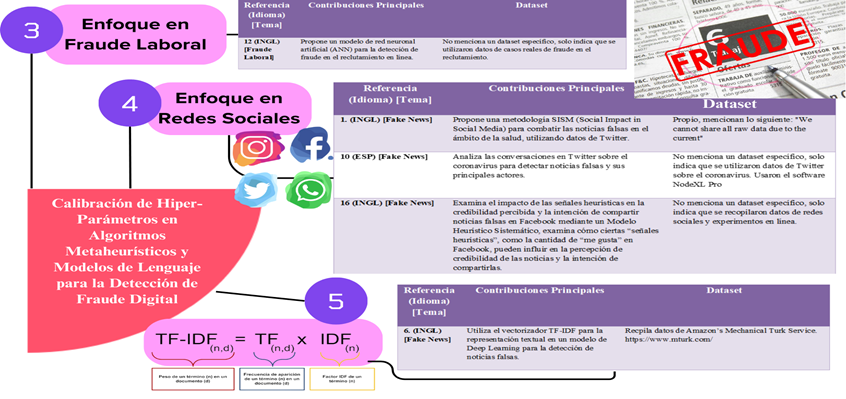
\includegraphics[width=\textwidth]{Imagenes/mapaConceptual4.png}
    \caption{Mapa Conceptual 4: Clasificación de artículos por enfoque.}
    \label{fig:mapa_conceptual_4}
\end{figure}

\section{Análisis del Impacto Social y Rol de los Medios}
Comprender el impacto social de la desinformación es crucial. Investigaciones como la de Singh et al. \cite{singh2023comprehensive} abordan la complejidad y los desafíos de la detección en redes sociales. Ali et al. \cite{ali2021fake} examinaron cómo heurísticas (como la cantidad de ``me gusta'') influyen en la credibilidad y la intención de compartir noticias en Facebook. El rol de los medios de comunicación es fundamental en esta lucha; trabajos como los de Ulloa et al. \cite{carcamo2021fake} y Pérez-Dasilva et al. \cite{perez2020fake} analizan cómo los medios en Chile, España y en el contexto de la pandemia de COVID-19 abordan la desinformación.

\section{Detección Aplicada a Fraude Financiero y Laboral}
El estado del arte se extiende a dominios críticos como el fraude financiero y laboral. Artículos como el de Cao et al. \cite{cao2020corporate} analizan cómo las decisiones de empleo pueden ser indicadores ("red flags") de riesgo de fraude financiero para los auditores. En el ámbito del fraude laboral, Nasser et al. \cite{nasser2021online} presentan un modelo basado en Redes Neuronales Artificiales (ANN) para detectar publicaciones de trabajo fraudulentas, mientras que Álvarez \cite{alvarez2021fraude} aborda las nuevas modalidades de fraude en la era digital en Latinoamérica. El Mapa Conceptual \ref{fig:mapa_conceptual_4} clasifica varios artículos según su enfoque en estas problemáticas.

\section{La Detección como un Problema de Optimización}
Varios trabajos abordan la detección como un problema de optimización. Aqil y Limam \cite{aqil2021modeling} lo modelan como un problema de planificación de tareas (\textit{Job Shop Scheduling}) y aplican tres metaheurísticas (IG, GA y ABC), concluyendo que IG supera a las demás. Por otro lado, Yazdi et al. \cite{yazdi2020improving} presentan una técnica de selección de características que combina K-means y SVM para reducir la dimensionalidad de los datos. El Mapa Conceptual \ref{fig:mapa_conceptual_5} resume varios de estos métodos.

\section{Algoritmos Metaheurísticos: Fundamentos y Aplicaciones}
\label{sec:algoritmos_metaheuristicos}

Los algoritmos metaheurísticos representan una clase de técnicas de optimización que han demostrado ser especialmente efectivas para resolver problemas complejos de optimización no lineal, incluyendo la calibración de hiperparámetros en modelos de aprendizaje automático. Esta sección presenta los fundamentos teóricos de los principales algoritmos metaheurísticos utilizados en la detección de noticias falsas y optimización de modelos.

\subsection{Algoritmos Genéticos (GA)}

Los Algoritmos Genéticos, introducidos por Holland \cite{holland1992adaptation}, están inspirados en la teoría de la evolución de Darwin y los principios de la genética. Estos algoritmos mantienen una población de soluciones candidatas que evolucionan a través de operadores genéticos como selección, cruzamiento y mutación. El trabajo seminal de Holland estableció las bases teóricas para esta clase de algoritmos bioinspirados, demostrando su capacidad para explorar eficientemente espacios de búsqueda complejos y multimodales.

El funcionamiento básico involucra la evaluación de la aptitud de cada individuo en la población, la selección de los mejores candidatos para reproducción, y la generación de nuevas soluciones mediante la combinación y modificación de las características de los padres. Este proceso iterativo permite la convergencia hacia soluciones óptimas o cerca del óptimo global.

\subsection{Optimización por Enjambre de Partículas (PSO)}

La Optimización por Enjambre de Partículas fue desarrollada por Kennedy y Eberhart \cite{kennedy1995particle}, inspirándose en el comportamiento social de bandadas de pájaros y bancos de peces. Una versión alternativa fue presentada por Eberhart y Kennedy \cite{eberhart1995particle} en el mismo período, consolidando esta técnica como una de las metaheurísticas más utilizadas.

En PSO, cada partícula representa una solución potencial que se mueve a través del espacio de búsqueda siguiendo su propia experiencia (mejor posición personal) y la experiencia del enjambre (mejor posición global). La velocidad y posición de cada partícula se actualizan dinámicamente, permitiendo un balance entre exploración y explotación del espacio de soluciones.

\subsection{Recocido Simulado y Métodos Multi-arranque}

El Recocido Simulado, propuesto por Kirkpatrick, Gelatt y Vecchi \cite{kirkpatrick1983optimization}, se basa en el proceso físico de enfriamiento controlado de metales. Este algoritmo permite escapar de óptimos locales mediante la aceptación probabilística de soluciones peores, con una probabilidad que disminuye gradualmente según un esquema de enfriamiento.

Los métodos Multi-arranque, formalizados por Martí, Resende y Pardalos \cite{marti2018multistart}, consisten en ejecutar múltiples corridas independientes de un algoritmo de búsqueda local desde diferentes puntos de inicio. La combinación de Recocido Simulado con estrategias Multi-arranque (MSA) permite aprovechar las ventajas de ambos enfoques: la capacidad de escape de óptimos locales del primero y la diversificación del segundo.

\subsection{Búsqueda Dispersa (Scatter Search)}

La Búsqueda Dispersa, desarrollada por Glover \cite{glover1998template}, utiliza estrategias sistemáticas para combinar soluciones de referencia y generar nuevas soluciones prometedoras. A diferencia de otros métodos que dependen de procesos aleatorios, SS emplea combinaciones determinísticas y diversificación controlada.

El algoritmo mantiene un conjunto de soluciones de referencia diversas y de alta calidad, utilizando métodos de combinación específicos del problema para generar nuevas soluciones. Esta aproximación ha demostrado ser particularmente efectiva en problemas de optimización combinatorial.

\subsection{Búsqueda en Vecindades Variables (VNS)}

La Búsqueda en Vecindades Variables, introducida por Mladenović y Hansen \cite{mladenovic1997variable}, se basa en el principio de cambio sistemático de estructuras de vecindad durante el proceso de búsqueda. Esta técnica es especialmente efectiva para escapar de óptimos locales explorando diferentes definiciones de vecindad.

VNS alterna entre fases de diversificación (mediante la exploración de vecindades más amplias) y intensificación (búsqueda local en vecindades más restringidas), proporcionando un marco flexible para la optimización que puede adaptarse a diferentes tipos de problemas.

\subsection{Aplicaciones en Detección de Noticias Falsas}

La Tabla \ref{tab:algoritmos_metaheuristicos} resume las características principales de estos algoritmos y sus aplicaciones específicas en el contexto de la detección de noticias falsas y optimización de modelos de aprendizaje automático.

\begin{table}[htbp]
\centering
\adjustbox{width=\textwidth,center}{%
\small
\begin{tabular}{|l|l|l|l|c|}
\hline
\rowcolor{UAMPurple!20}
\textbf{Algoritmo} & \textbf{Inspiración} & \textbf{Características Principales} & \textbf{Aplicaciones en Detección} & \textbf{Ref.} \\
\hline
\begin{tabular}[t]{@{}l@{}}Algoritmos Genéticos\\(GA)\end{tabular} & \begin{tabular}[t]{@{}l@{}}Evolución biológica\\y genética\end{tabular} & \begin{tabular}[t]{@{}l@{}}Población de soluciones,\\operadores genéticos,\\selección natural\end{tabular} & \begin{tabular}[t]{@{}l@{}}Optimización de hiperparámetros,\\selección de características,\\arquitecturas de redes neuronales\end{tabular} & \cite{holland1992adaptation} \\
\hline
\begin{tabular}[t]{@{}l@{}}Optimización por\\Enjambre de Partículas\\(PSO)\end{tabular} & \begin{tabular}[t]{@{}l@{}}Comportamiento\\social de bandadas\\y enjambres\end{tabular} & \begin{tabular}[t]{@{}l@{}}Partículas con velocidad\\y posición, memoria\\personal y social\end{tabular} & \begin{tabular}[t]{@{}l@{}}Calibración de pesos en redes,\\optimización de parámetros\\de modelos de lenguaje\end{tabular} & \cite{kennedy1995particle} \\
\hline
\begin{tabular}[t]{@{}l@{}}Recocido Simulado\\(SA)\end{tabular} & \begin{tabular}[t]{@{}l@{}}Proceso físico de\\enfriamiento de metales\end{tabular} & \begin{tabular}[t]{@{}l@{}}Aceptación probabilística,\\esquema de enfriamiento,\\escape de óptimos locales\end{tabular} & \begin{tabular}[t]{@{}l@{}}Optimización de arquitecturas\\profundas, ajuste fino\\de modelos complejos\end{tabular} & \cite{kirkpatrick1983optimization} \\
\hline
\begin{tabular}[t]{@{}l@{}}Multi-arranque\\(Multi-start)\end{tabular} & \begin{tabular}[t]{@{}l@{}}Diversificación\\de puntos de inicio\end{tabular} & \begin{tabular}[t]{@{}l@{}}Múltiples ejecuciones\\independientes, exploración\\global del espacio\end{tabular} & \begin{tabular}[t]{@{}l@{}}Inicialización robusta\\de modelos, validación\\cruzada optimizada\end{tabular} & \cite{marti2018multistart} \\
\hline
\begin{tabular}[t]{@{}l@{}}Búsqueda Dispersa\\(SS)\end{tabular} & \begin{tabular}[t]{@{}l@{}}Combinación sistemática\\de soluciones diversas\end{tabular} & \begin{tabular}[t]{@{}l@{}}Conjunto de referencia,\\combinaciones determinísticas,\\diversificación controlada\end{tabular} & \begin{tabular}[t]{@{}l@{}}Ensemble de modelos,\\combinación de características,\\optimización de pipelines\end{tabular} & \cite{glover1998template} \\
\hline
\begin{tabular}[t]{@{}l@{}}Búsqueda en Vecindades\\Variables (VNS)\end{tabular} & \begin{tabular}[t]{@{}l@{}}Cambio sistemático\\de estructuras de\\vecindad\end{tabular} & \begin{tabular}[t]{@{}l@{}}Múltiples definiciones\\de vecindad, alternancia\\entre diversificación\\e intensificación\end{tabular} & \begin{tabular}[t]{@{}l@{}}Exploración de espacios\\de hiperparámetros,\\optimización de topologías\\de red\end{tabular} & \cite{mladenovic1997variable} \\
\hline
\end{tabular}
}
\caption{Algoritmos metaheurísticos: características y aplicaciones en detección de noticias falsas.}
\label{tab:algoritmos_metaheuristicos}
\end{table}

Estos algoritmos han demostrado ser especialmente valiosos en el contexto de la detección de noticias falsas, donde los espacios de búsqueda de hiperparámetros son complejos y multidimensionales. Su capacidad para balancear exploración y explotación los convierte en herramientas ideales para optimizar el rendimiento de modelos de aprendizaje automático en tareas de clasificación textual.

\begin{figure}[h!]
    \centering
    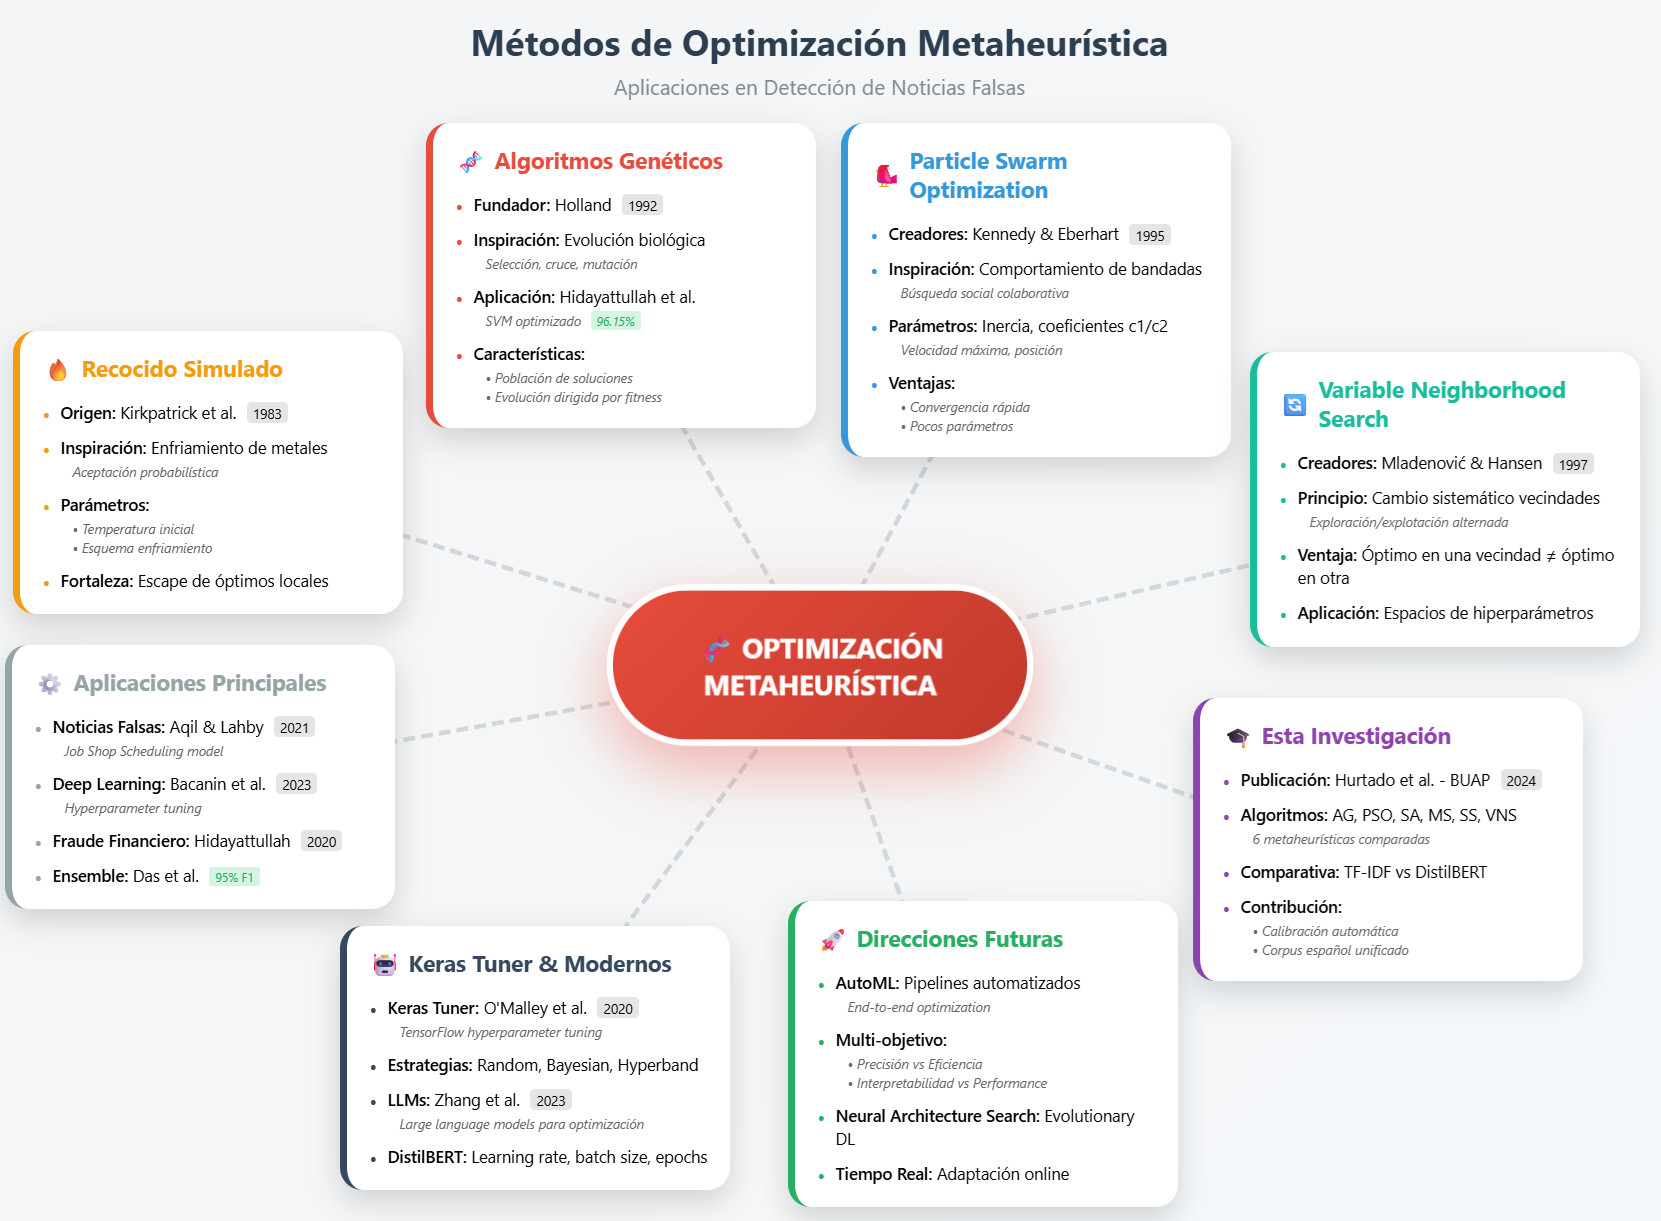
\includegraphics[width=\textwidth]{Imagenes/mapaConceptual5.png}
    \caption{Mapa Conceptual 5: Métodos para resolver la problemática presentados en los artículos.}
    \label{fig:mapa_conceptual_5}
\end{figure}



\section{El Rol de los Modelos de Lenguaje}
Los modelos de lenguaje son centrales en la detección moderna. Como se muestra en el Mapa Conceptual \ref{fig:mapa_conceptual_6}, enfoques como el de Das et al. \cite{das2022heuristic} combinan modelos pre-entrenados como BERT con algoritmos heurísticos que incorporan atributos de las noticias (fuente, URL, autor) como características estadísticas. Otros trabajos se centran en el análisis textual cualitativo para descubrir significados latentes \cite{ali2020posttruth} o utilizan metaheurísticas para optimizar el procesamiento de documentos \cite{aqil2021modeling}.

\section{Hiperparámetros en Modelos de Aprendizaje Automático}
\label{sec:hiperparametros}

\subsection{¿Qué son los Hiperparámetros?}

Para explicar este concepto de la manera más sencilla, utilizaremos una analogía: cocinar un pastel.

Imagina que estás construyendo un modelo de machine learning (el pastel).

Los \textbf{parámetros} son los elementos que el modelo aprende por sí mismo durante el entrenamiento (la cocción). Por ejemplo, cómo se combinan la harina y el azúcar dentro del horno. En una red neuronal, estos son los pesos (\textit{weights}) y sesgos (\textit{biases}) de las neuronas. No los eliges tú directamente, se ajustan solos a partir de los datos.

Los \textbf{hiperparámetros}, en cambio, son las decisiones que tú tomas antes de empezar a entrenar. Son los ajustes o ``perillas'' de la receta que tú, como cocinero (científico de datos), debes fijar. Por ejemplo:

\begin{itemize}
    \item \textbf{La temperatura del horno} → tasa de aprendizaje (\textit{learning rate})
    \item \textbf{El tiempo de cocción} → número de épocas
    \item \textbf{La cantidad de cada ingrediente principal} → número de capas o neuronas
    \item \textbf{El tipo de molde} → arquitectura del modelo
\end{itemize}

Si eliges mal estos ajustes, tu pastel puede quemarse (sobreajuste u \textit{overfitting}), quedar crudo (subajuste o \textit{underfitting}), o simplemente no tener buen sabor (bajo rendimiento).

\subsection{¿Por qué son Importantes en la Detección de Noticias Falsas?}

En el contexto de la detección de noticias falsas, elegir los hiperparámetros correctos es crucial porque:

\begin{itemize}
    \item Los textos en español tienen características lingüísticas específicas que requieren configuraciones particulares
    \item Los patrones de desinformación pueden ser muy sutiles y necesitan modelos finamente ajustados
    \item Una mala configuración puede hacer que el modelo confunda sarcasmo con falsedad, o que no detecte desinformación sofisticada
\end{itemize}

\subsection{El Problema: Encontrar la Mejor Configuración}

Tradicionalmente, los científicos de datos probaban diferentes combinaciones de hiperparámetros manualmente o usando métodos como:

\begin{itemize}
    \item \textbf{Búsqueda en grilla (Grid Search)}: Probar todas las combinaciones posibles - muy lento
    \item \textbf{Búsqueda aleatoria (Random Search)}: Probar combinaciones al azar - más eficiente pero sin dirección
\end{itemize}

Aquí es donde entran los algoritmos metaheurísticos, que son como ``cocineros inteligentes'' que aprenden de cada pastel que hacen para mejorar la siguiente receta.

\subsection{Herramientas Modernas: Keras Tuner}

En el ecosistema de TensorFlow, Keras Tuner \cite{omalley2020hyperparameter} ha emergido como una herramienta fundamental para automatizar la búsqueda de los mejores hiperparámetros. Desarrollado por el equipo de Keras, esta biblioteca permite que el sistema pruebe automáticamente diferentes ``recetas'' y encuentre la mejor configuración para tu modelo.

Keras Tuner facilita:
\begin{itemize}
    \item Definir fácilmente qué hiperparámetros quieres optimizar
    \item Probar múltiples configuraciones en paralelo
    \item Monitorear el progreso en tiempo real
    \item Guardar y recuperar los mejores resultados
\end{itemize}

\subsection{La Ventaja de Combinar Modelos de Lenguaje con Keras Tuner}

Los modelos de lenguaje modernos como DistilBERT, cuando se combinan con herramientas como Keras Tuner, actúan como sistemas inteligentes que:

\begin{itemize}
    \item Aprenden representaciones semánticas complejas del texto
    \item Se benefician de la optimización automática de hiperparámetros
    \item Pueden encontrar configuraciones óptimas de manera más eficiente que los métodos manuales
    \item Balancean entre el aprendizaje de características profundas (exploración) y el ajuste fino de parámetros específicos (explotación)
\end{itemize}

En contraste, la búsqueda de parámetros en los algoritmos metaheurísticos se realiza de manera más tradicional, donde cada algoritmo implementa su propia estrategia de exploración del espacio de hiperparámetros sin depender de herramientas de automatización externas.

Esta combinación es especialmente poderosa para la detección de noticias falsas, donde la optimización automática puede significar la diferencia entre un modelo que apenas funciona y uno que detecta desinformación con alta precisión, aprovechando al máximo las capacidades semánticas de los transformers pre-entrenados.

\begin{figure}[h!]
    \centering
    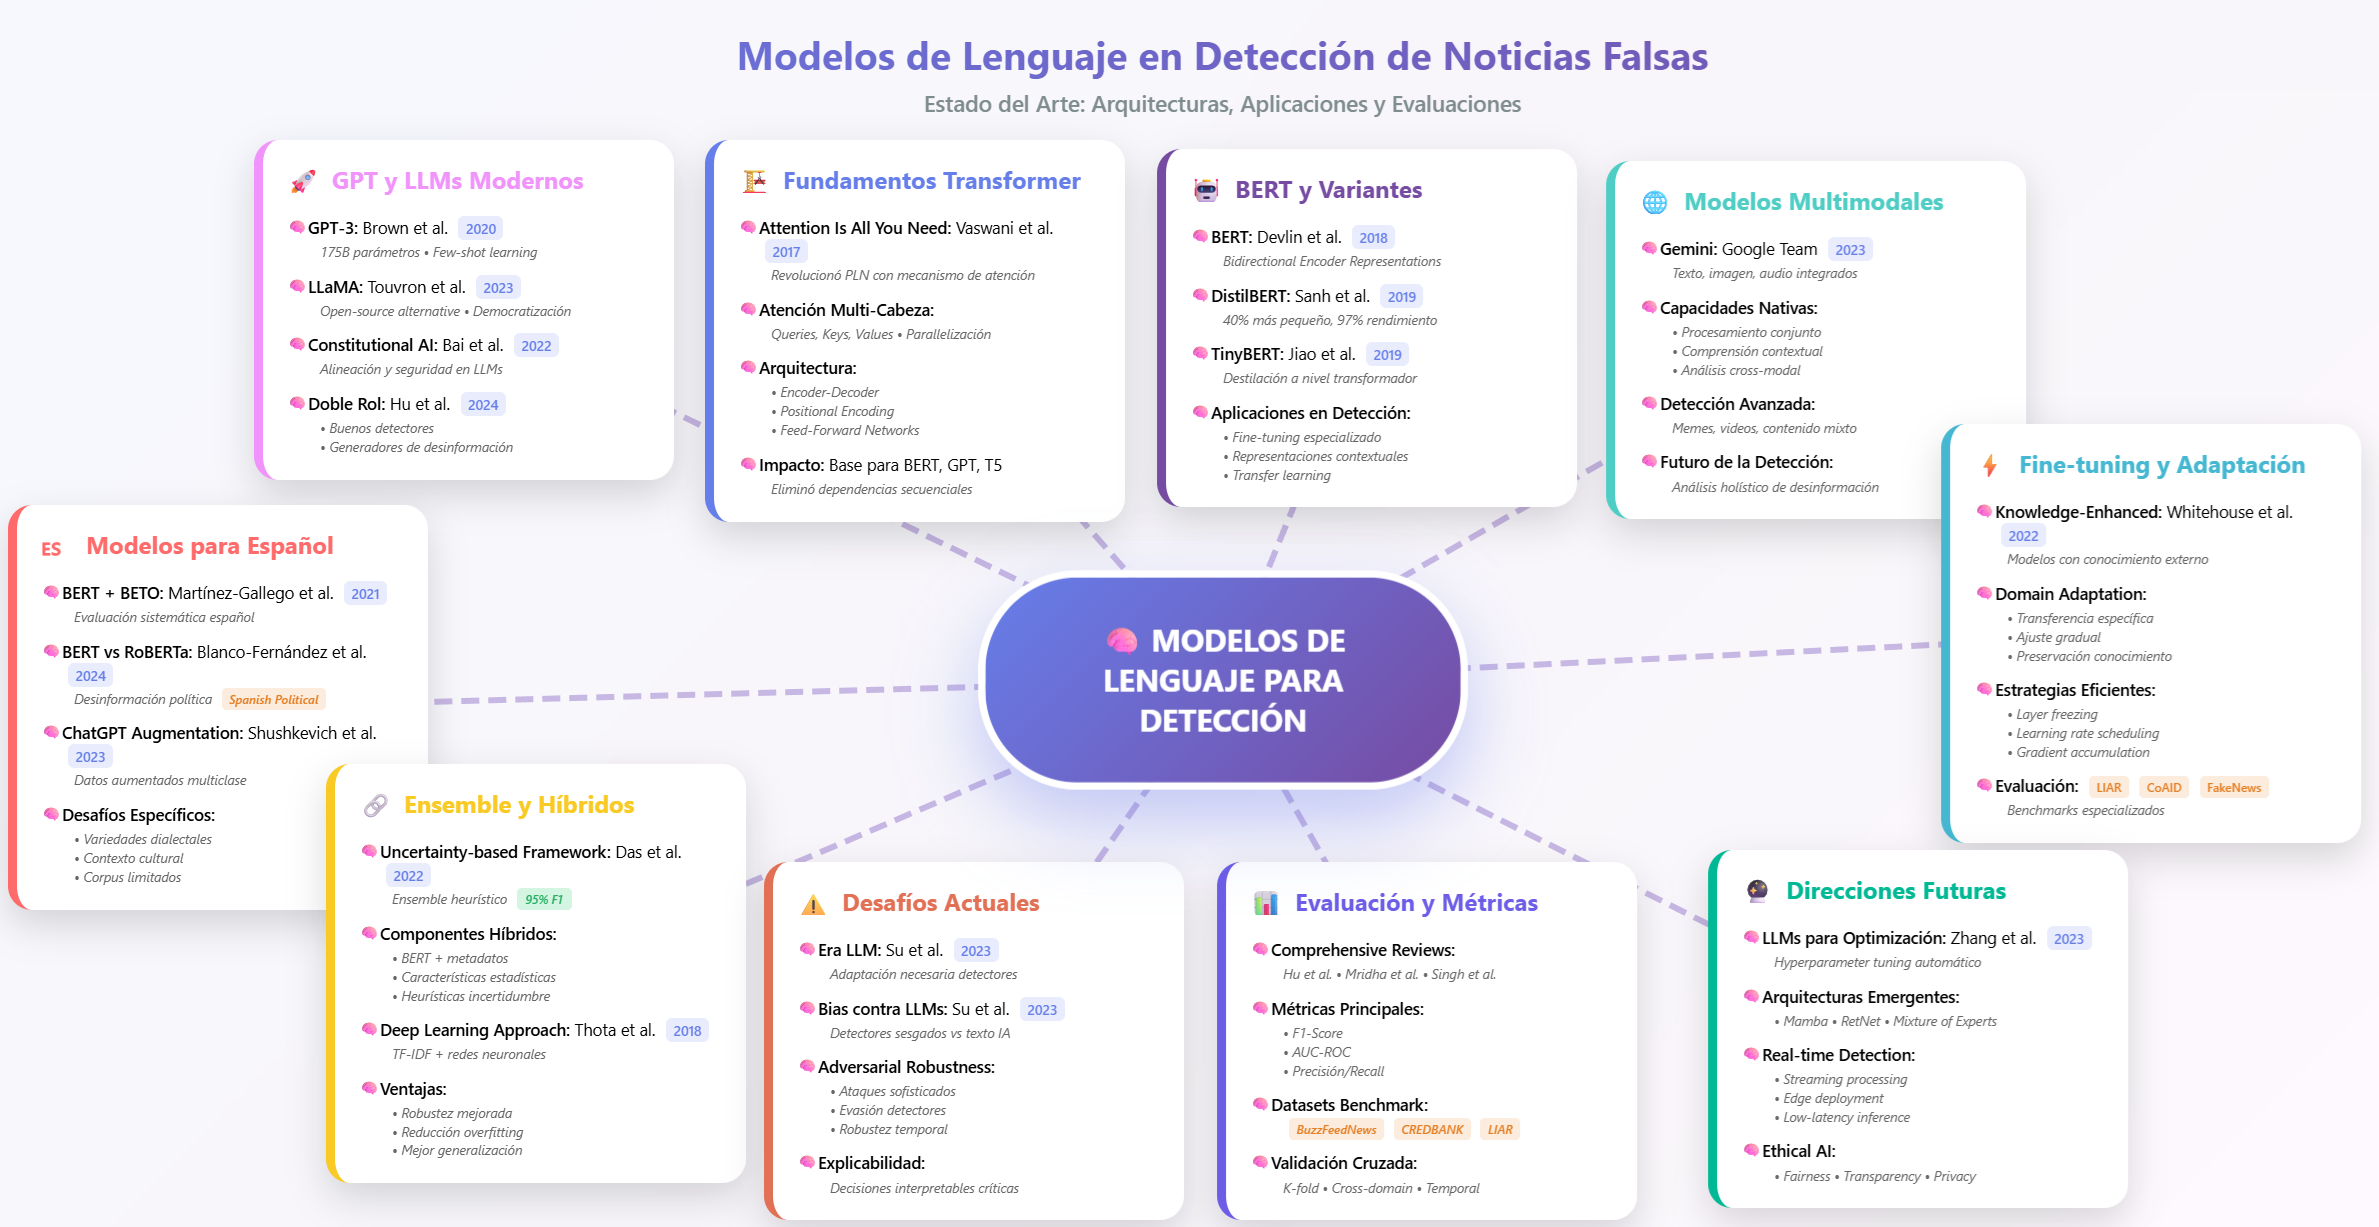
\includegraphics[width=\textwidth]{Imagenes/mapaConceptual6.png}
    \caption{Mapa Conceptual 6: Artículos relacionados que incorporan Modelos de Lenguaje.}
    \label{fig:mapa_conceptual_6}
\end{figure}

\section{Síntesis y Perspectivas Futuras}
\label{sec:sintesis_perspectivas}

La revisión comprehensiva de la literatura revela una evolución clara en las aproximaciones para la detección de noticias falsas y fraude digital. Desde los primeros enfoques basados en características lingüísticas hasta los modernos sistemas basados en transformers y LLMs, el campo ha experimentado avances significativos en términos de precisión y escalabilidad.

Los desafíos identificados incluyen: (1) la necesidad de mayor cantidad de datos etiquetados en español, (2) la adaptación de modelos a contextos culturales específicos, (3) la optimización eficiente de hiperparámetros en modelos complejos, y (4) la integración de información multimodal y conocimiento externo. Esta tesis contribuye especialmente a los puntos (1) y (3) mediante la unificación de corpus existentes y la aplicación de técnicas metaheurísticas para la optimización de modelos de detección.

La organización temática presentada en este capítulo proporciona un marco comprehensivo para entender las diferentes dimensiones del problema y justifica la aproximación metodológica híbrida adoptada en esta investigación, combinando modelos de lenguaje state-of-the-art con técnicas de optimización metaheurística.